\chapter{Updatable Vector Tiles}

\osm{} contributors add more than $3\,000\,000$ nodes and $3\,000\,000$ ways every day.
In order to keep the prerendered tiles up to data this poses a challenge of looking at the changes
and figuring out which tiles are affected by those changes and schedule them for rerendering.


\begin{listing}[H]
  \centering
  \begin{xmlcode}
<?xml version='1.0' encoding='UTF-8'?>
<osmChange version="0.6" timestamp="2016-04-03T00:00:00Z">
<modify>
    <node id="1" lat="47.4918119" lon="19.0449869" version="2"
          timestamp="2016-04-01T00:00:11Z" changeset="1" uid="1" user="o2v">
        <tag k="name" v="n1-place-neighbourhood-UPDATED!!!!!"/>
        <tag k="place" v="neighbourhood"/>
    </node>
</modify>
</osmChange>
  \end{xmlcode}
  \caption{}
\end{listing}


\subchapter{Track changes}

\osm{} does not contain real geometry but only three data types. Points, ways and relations.
The actual geometries are created by imposm3.

\subchapter{Track deleted rows}

For each table the \texttt{track\_osm\_delete} trigger is enabled to keep track of deleted rows.

\begin{listing}[H]
  \centering
  \begin{sqlcode}
    DROP TRIGGER IF EXISTS osm_building_polygon_track_delete ON osm_building_polygon;
    CREATE TRIGGER osm_building_polygon_track_delete
    BEFORE DELETE ON osm_building_polygon
    FOR EACH ROW EXECUTE PROCEDURE track_osm_building_polygon_delete()
  \end{sqlcode}
  \caption{}
\end{listing}

The trigger will track the delete in a separate table before discarding it.

\begin{listing}[H]
  \centering
  \begin{sqlcode}
CREATE OR REPLACE FUNCTION track_osm_building_polygon_delete() returns TRIGGER
AS $$
BEGIN
     IF (TG_OP = 'DELETE') THEN
        INSERT INTO osm_building_polygon_delete(id, geometry)
        VALUES($1, $2) USING OLD.id, OLD.geometry;
        RETURN OLD;
     END IF;

     RETURN NULL;
END;
$$ language plpgsql;
  \end{sqlcode}
  \caption{}
\end{listing}


\subchapter{Calculate changed tiles}

\section{Criterias}\label{criterias}

\paragraph{Speed} 
The detection of affected tiles must be as fast as possible. 
The goal is to apply updates of \osm{} within one day. If the dirty tiles detection
already takes longer than that it is no longer possible to keep up with \osm{} updates.

\paragraph{Single Source of Truth}

In both approaches if a query in the data style has been changed it shouldn't be necessary
to edit the code in multiple places to support that change to keep it maintainable.


\section{Recursive tile matching of Geometry}

Given a Polygon the fastest way to determine which tiles are covered by a geometry is to recursively descend and check which tiles are affected.

\subsubsection*{Algorithm}

\begin{enumerate}  
    \item Calculate the extent for a given XYZ tile index
    \item Match the geometry with the tile extent making full use of the GIST index on the geometry
    \item Select the matches
    \item Recursively descend for all children of the matching tiles
\end{enumerate}

\begin{figure}[H]
  \centering
  \includegraphics[width=0.9\textwidth]{images/polygon_xyz_matching.png}
  \caption{Recursive tile matching on polygon}
\end{figure}

\subsubsection*{Support Tile Buffer}

Vector tiles are utilizing tile buffers to ensure nice geometry joining. To support this a buffer can be added to the XYZ extent of a tile.

\begin{figure}[H]
  \centering
  \includegraphics[width=0.7\textwidth]{images/polygon_buffer_xyz_matching.png}
  \caption{Recursive buffered tile matching on polygon}
\end{figure}


\subsubsection*{PostgreSQL Implementation}

\begin{listing}[H]
  \centering
  \begin{sqlcode}
CREATE OR REPLACE FUNCTION overlapping_tiles(
    geom geometry,
    max_zoom_level INTEGER,
    buffer_size INTEGER
) RETURNS TABLE (
    tile_z INTEGER,
    tile_x INTEGER,
    tile_y INTEGER
) AS $$
BEGIN
    RETURN QUERY
        WITH RECURSIVE tiles(x, y, z, e) AS (
            SELECT 0, 0, 0, geom && XYZ_Extent(0, 0, 0, buffer_size)
            UNION ALL
            SELECT x*2 + xx, y*2 + yy, z+1,
                   geom && XYZ_Extent(x*2 + xx, y*2 + yy, z+1, buffer_size)
            FROM tiles,
            (VALUES (0, 0), (0, 1), (1, 1), (1, 0)) as c(xx, yy)
            WHERE e AND z < max_zoom_level
        )
        SELECT z, x, y FROM tiles WHERE e;
END;
$$ LANGUAGE plpgsql IMMUTABLE;
  \end{sqlcode}
  \caption{Recursive tile matching of geometry}
\end{listing}


\section{Point Optimization}

Points only occur in one tile at each zoom level (neglecting tile buffers). 

\begin{figure}[H]
  \centering
  \includegraphics[width=0.9\textwidth]{images/point_xyz_matching.png}
  \caption{Tiles covering a point geometry}
\end{figure}

Therefore given a point we can immediately calculate the tile it is covering saving the recursive descend.
To neglect overhead of PostgreSQL dynamic language a PostgreSQL C extension has been written which improves tile calculation for points a hundred fold.

\begin{listing}[H]
  \centering
  \begin{ccode}
#include "math.h"
float8 D2R = M_PI / 180.0;

// Latitude and longitude of Zurich
int32 zoom_level = 14;
float8 lat = 47.376887;
float8 lon = 8.541694;

float8 _sin = sin(lat * D2R);
float8 z2 = pow(2, zoom_level);

// XYZ Tile index calculated from latitude and longitude
int32 x = floor(z2 * (lon / 360 + 0.5));
int32 y = floor(z2 * (0.5 - 0.25 * log((1 + _sin) / (1 - _sin)) / M_PI));

  \end{ccode}
  \caption{Calculate tile at given zoom level for a point}
\end{listing}

Applying the \texttt{overlapping\_tiles} function over millions of polygons is very efficient thanks to the new \texttt{LATERAL} join type.

\begin{listing}[H]
  \centering
  \begin{sqlcode}
    SELECT DISTINCT t.tile_x AS x, t.tile_y AS y, t.tile_z AS z
    FROM osm_building_polygon AS g
    INNER JOIN LATERAL overlapping_tiles(g.geometry, 14, 4) AS t ON true
  \end{sqlcode}
  \caption{Calculate all tiles covered by building polygons}
\end{listing}

\begin{figure}[H]
  \centering
  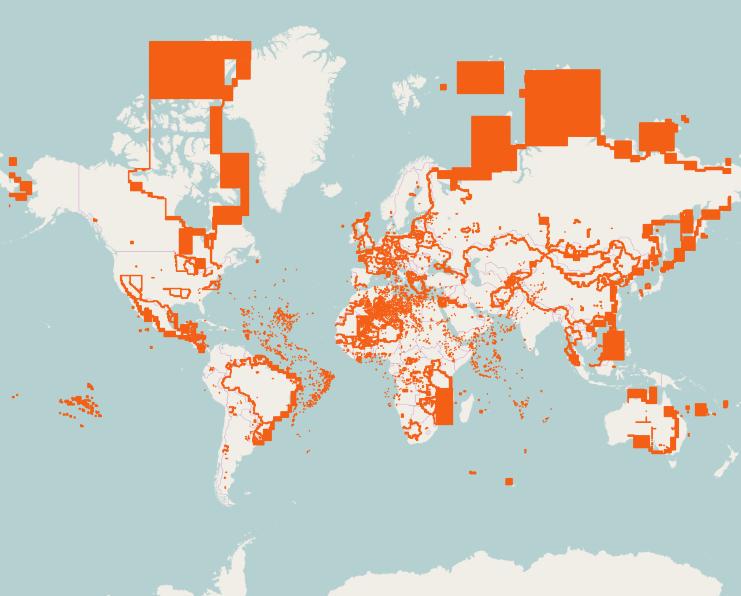
\includegraphics[width=1\textwidth]{images/changed_tiles_z10.png}
  \caption{Changed tiles on z10 over course of 10 days}
\end{figure}
